\chapter{外微分形式与积分定理}

\section{从向量分析到微分形式}

前两章已经使用曲线坐标、度规张量和协变导数重新表述了向量分析中的梯度、散度、旋度和拉普拉斯算子. 这种语言已经能够处理一般曲线坐标中的计算问题. 

从更高层次看, 传统向量分析中的许多公式其实具有共同结构. 例如: 
\[
\nabla\times(\nabla f)=0,
\]
\[
\nabla\cdot(\nabla\times\bm{A})=0,
\]
以及Gauss公式和Stokes公式: 
\[
\int_V\nabla\cdot\bm{A}\,\dif V
=
\oint_{\partial V}\bm{A}\cdot \dif\bm{S},
\]
\[
\int_S(\nabla\times\bm{A})\cdot \dif\bm{S}
=
\oint_{\partial S}\bm{A}\cdot \dif\bm{l}.
\]
这些公式形式上分别涉及标量场、向量场、面积分和线积分, 但它们本质上都来自同一个结构: 外微分与边界积分之间的关系. 

微分形式的作用在于用统一语言描述不同维数积分中的被积对象及其微分关系. 具体而言, 线积分对应一次形式, 面积分对应二次形式, 体积分对应三次形式; 相应地, 标量场可视为零次形式. 

在三维空间中, $0$-形式、$1$-形式、$2$-形式和 $3$-形式分别对应标量场、线积分对象、通量面积分对象和体积分密度. 

微分形式的优势在于: 它直接适合积分, 不需要先把对象解释成“向量”再人为区分线元、面积元和体积元. 

\section{切空间、余切空间与一次形式}

设空间中的一点为 $p$. 在该点处, 所有切向量构成一个向量空间, 称为切空间, 记为
\[
T_pM.
\]
如果使用局部坐标
\[
(x^1,x^2,x^3),
\]
则切空间的一组自然基底为
\begin{equation}\label{eq:3.1}
	\frac{\partial}{\partial x^1},
\qquad
\frac{\partial}{\partial x^2},
\qquad
\frac{\partial}{\partial x^3}.
\end{equation}
通常简写为
\[
\partial_i=\frac{\partial}{\partial x^i}.
\]
于是任意切向量可以写成
\[
X=X^i\partial_i.
\]
\begin{figure}[h]
	\centering
	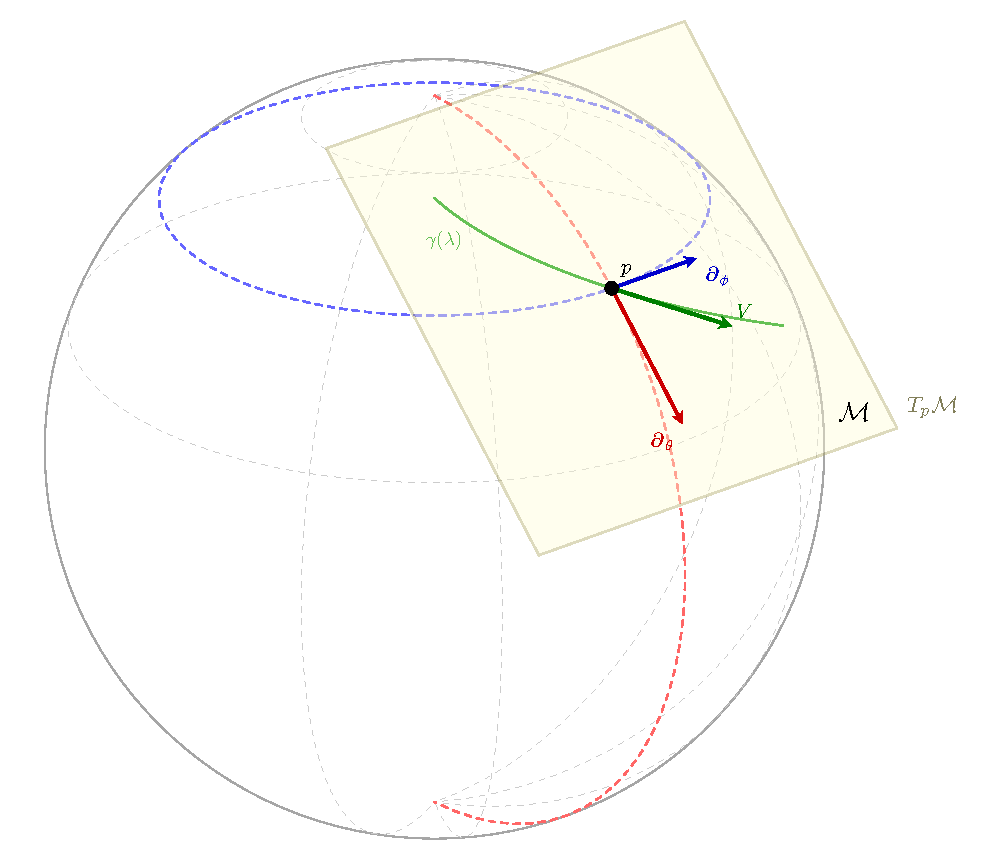
\includegraphics[width=0.75\linewidth]{figure/fig3.1}
	\caption[球面上的切空间和曲线上的切矢量]{球面$S^2$上的切空间和曲线上的切矢量}
	\label{fig:3.1}
\end{figure}

与切空间对偶的是余切空间, 记为
\[
T_p^*M.
\]
余切空间中的元素称为协向量, 或一次微分形式. 它们是作用在切向量上的线性函数. 

局部坐标下, 余切空间的自然基底为
\[
\dif x^1,\dif x^2,\dif x^3.
\]
它们与切空间基底满足对偶关系: 
\begin{equation}\label{eq:3.2}
	\dif x^i(\partial_j)=\delta^i_j.
\end{equation}
因此, 任意一次形式可以写成
\[
\omega=\omega_i \dif x^i.
\]
若切向量为
\[
X=X^i\partial_i,
\]
则一次形式 $\omega$ 作用在 $X$ 上得到
\[
\omega(X)
=
\omega_i \dif x^i(X^j\partial_j).
\]
利用线性性和对偶关系, 有
\[
\omega(X)
=
\omega_iX^j\dif x^i(\partial_j)
=
\omega_iX^j\delta^i_j.
\]
因此
\[
\omega(X)=\omega_iX^i.
\]
这说明一次形式天然适合与向量配对, 并给出标量. 

\section{标量场的微分}

设 $f$ 是一个标量场. 它的外微分, 也就是普通微分, 定义为
\[
\dif f=\partial_i f\,\dif x^i.
\]
对于任意切向量
\[
X=X^i\partial_i,
\]
有
\[
\dif f(X)
=
\partial_i f\,\dif x^i(X^j\partial_j)
=
\partial_i f\,X^i.
\]
这正是函数 $f$ 沿方向 $X$ 的方向导数: 
\[
X(f)=X^i\partial_i f.
\]
因此, $\dif f$ 的几何意义是: 它把任意方向 $X$ 映射为函数 $f$ 沿该方向的变化率. 

需要注意的是, $\dif f$ 是一次形式, 不是向量. 只有引入度规以后, 才能通过度规把一次形式 $\dif f$ 对应到梯度向量 $\nabla f$. 

在欧氏空间中, 二者通过
\[
\dif f(X)=\nabla f\cdot X
\]
联系起来. 

用指标表示, 若
\[
\nabla f=(\nabla f)^i\bm{e}_i,
\]
则
\[
(\nabla f)^i=g^{ij}\partial_j f.
\]
因此
\[
\nabla f
=
g^{ij}\partial_j f\,\bm{e}_i.
\]
而 $\dif f$ 本身始终是
\[
\dif f=\partial_i f\,\dif x^i.
\]
由此可见, 外微分 $\dif$ 不需要度规, 而梯度 $\nabla f$ 需要度规. 

\section{外积与反对称性}

为了描述有向面积元和体积元, 需要引入外积. 外积记为
\[
\wedge.
\]
对一次形式 $\dif x^i$ 和 $\dif x^j$, 外积满足反对称性: 
\begin{equation}\label{eq:3.3}
	\dif x^i\wedge \dif x^j=-\dif x^j\wedge \dif x^i.
\end{equation}
特别地, 
\[
\dif x^i\wedge \dif x^i=0.
\]
这表示两个相同方向不能张成非零面积. 

一个二次形式可以写成
\[
\omega
=
\frac{1}{2}\omega_{ij}\dif x^i\wedge \dif x^j.
\]
由于
\[
\dif x^i\wedge \dif x^j=-\dif x^j\wedge \dif x^i,
\]
只有 $\omega_{ij}$ 的反对称部分真正起作用. 因此通常要求
\[
\omega_{ij}=-\omega_{ji}.
\]
在三维空间中, 典型的二次形式为
\[
\omega
=
\omega_{12}\dif x^1\wedge \dif x^2
+
\omega_{23}\dif x^2\wedge \dif x^3
+
\omega_{31}\dif x^3\wedge \dif x^1.
\]
它适合在二维曲面上积分. 

三次形式可以写成
\[
\Omega
=
F\,\dif x^1\wedge \dif x^2\wedge \dif x^3.
\]
它适合在三维区域上积分. 

更一般地, 在 $n$ 维空间中, $p$-形式可以写成
\[
\omega
=
\frac{1}{p!}\omega_{i_1i_2\cdots i_p}
\dif x^{i_1}\wedge \dif x^{i_2}\wedge\cdots\wedge \dif x^{i_p},
\]
其中分量 $\omega_{i_1i_2\cdots i_p}$ 对所有指标完全反对称. 

\section{外微分算子}

外微分算子 $\dif$ 把 $p$-形式映射为 $(p+1)$-形式: 
\[
\dif:\Lambda^p\to\Lambda^{p+1}.
\]
对标量函数 $f$, 有
\[
\dif f=\partial_i f\,\dif x^i.
\]
对一次形式
\[
\omega=\omega_i \dif x^i,
\]
其外微分定义为
\[
\dif\omega
=
\partial_j\omega_i\,\dif x^j\wedge \dif x^i.
\]
利用外积的反对称性, 可以写成标准形式: 
\[
\dif\omega
=
\frac{1}{2}
(\partial_i\omega_j-\partial_j\omega_i)
\dif x^i\wedge \dif x^j.
\]
这里第二步来自交换哑指标并利用
\[
\dif x^j\wedge \dif x^i=-\dif x^i\wedge \dif x^j.
\]
对二次形式
\[
\eta
=
\frac{1}{2}\eta_{ij}\dif x^i\wedge \dif x^j,
\]
其外微分为
\[
\dif\eta
=
\frac{1}{2}\partial_k\eta_{ij}
\dif x^k\wedge \dif x^i\wedge \dif x^j.
\]
等价地, 可以写成完全反对称形式: 
\[
\dif\eta
=
\frac{1}{3!}
(\partial_i\eta_{jk}
+
\partial_j\eta_{ki}
+
\partial_k\eta_{ij})
\dif x^i\wedge \dif x^j\wedge \dif x^k.
\]
在三维空间中, 三次形式已经是最高阶形式, 因此对任意三次形式 $\Omega$, 有
\[
\dif\Omega=0.
\]
\section{外微分的幂零性}

外微分最重要的代数性质是幂零性: 
\[
\dif^{2}=0.
\]
这表示连续作用两次外微分必定为零. 

先看标量函数 $f$. 有
\[
\dif f=\partial_i f\,\dif x^i.
\]
继续求外微分: 
\[
\dif(\dif f)
=
\partial_j\partial_i f\,\dif x^j\wedge \dif x^i.
\]
由于普通偏导满足
\[
\partial_j\partial_i f=\partial_i\partial_j f,
\]
而外积满足
\[
\dif x^j\wedge \dif x^i=-\dif x^i\wedge \dif x^j,
\]
对称的系数与反对称的基形式相乘后为零. 因此
\[
\dif^{2}f=0.
\]
这对应向量分析中的恒等式: 
\[
\nabla\times(\nabla f)=0.
\]
再看一次形式
\[
\omega=\omega_i \dif x^i.
\]
它的外微分是二次形式 $\dif\omega$. 继续作用 $\dif$, 由于二阶偏导的对称性与外积的完全反对称性, 仍然得到
\[
\dif(\dif\omega)=0.
\]
这对应向量分析中的恒等式: 
\[
\nabla\cdot(\nabla\times\bm{A})=0.
\]
因此, 两条熟悉的向量分析恒等式在微分形式语言中统一为一个公式: 
\[
\dif^{2}=0.
\]
\begin{example}{外微分的幂零性}{3,2}
设二维区域上的一次形式为
\[
\omega=P(x,y)\,\dif x+Q(x,y)\,\dif y.
\]
验证 $\dif^{2}\omega=0$. 
\end{example}
\begin{solution}
由外微分定义可得
\[
\dif\omega
=
(Q_x-P_y)\,\dif x\wedge\dif y.
\]
继续作用外微分, 得到
\[
\dif(\dif\omega)
=
\dif(Q_x-P_y)\wedge\dif x\wedge\dif y.
\]
而
\[
\dif(Q_x-P_y)
=
(Q_{xx}-P_{yx})\,\dif x+(Q_{xy}-P_{yy})\,\dif y.
\]
由于
\[
\dif x\wedge\dif x=0,
\qquad
\dif y\wedge\dif y=0,
\]
两项均为零, 因此
\[
\dif^{2}\omega=0.
\]
这正是外微分幂零性在一次形式上的具体表现. 
\end{solution}
\section{度规、体积形式与 Hodge 星算子}

外微分 $\dif$ 本身不依赖度规. 但是, 如果要把微分形式与传统向量分析中的梯度、旋度、散度联系起来, 就需要度规. 

度规给出长度、夹角和体积元. 设三维空间的度规为
\[
g_{ij},
\]
其行列式为
\[
g=\det(g_{ij}).
\]
定向体积形式为
\[
\mathrm{vol}
=
\sqrt{g}\,\dif x^1\wedge \dif x^2\wedge \dif x^3.
\]
Hodge 星算子 $*$ 依赖度规和取向. 它把 $p$-形式变成 $(3-p)$-形式: 
\[
*:\Lambda^p\to\Lambda^{3-p}.
\]
在三维欧氏空间中, 它的作用可以理解为: 把一个有向 $p$ 维元素变成与之正交的有向 $(3-p)$ 维元素. 

例如, 在笛卡尔正交归一坐标中, 有
\[
\begin{aligned}
	*1=&\dif x\wedge \dif y\wedge \dif z,\\
	*\dif x&=\dif y\wedge \dif z,\\
	*\dif y&=\dif z\wedge \dif x,\\
	*\dif z&=\dif x\wedge \dif y,
\end{aligned}
\]
以及
\[
\begin{aligned}
	*(\dif x\wedge \dif y)&=\dif z,\\
	*(\dif y\wedge \dif z)&=\dif x,\\
	*(\dif z\wedge \dif x)&=\dif y,
\end{aligned}
\]
最后还有
\[
*(\dif x\wedge \dif y\wedge \dif z)=1.
\]
在一般曲线坐标中, Hodge 星号的表达式会包含度规 $g_{ij}$ 和 $\sqrt{g}$. 因此, $\dif$ 是纯微分结构, 而 $*$ 反映度规结构. 

这一点非常关键: 旋度和散度之所以需要度规, 是因为它们都涉及把不同阶数的微分形式相互对应. 

\section{向量与微分形式的对应}

在带度规的三维空间中, 可以把向量和一次形式对应起来. 若
\[
\bm{A}=A^i\bm{e}_i,
\]
则它对应的一次形式记为
\[
A^\flat.
\]
定义为
\[
A^\flat
=
A_i \dif x^i,
\]
其中
\[
A_i=g_{ij}A^j.
\]
符号 $\flat$ 表示用度规降低指标, 把向量变成一次形式. 

反过来, 若有一次形式
\[
\omega=\omega_i \dif x^i,
\]
则可以通过升指标得到对应的向量
\[
\omega^\sharp
=
\omega^i\bm{e}_i,
\]
其中
\[
\omega^i=g^{ij}\omega_j.
\]
符号 $\sharp$ 表示用度规升高指标, 把一次形式变成向量. 

有了这个对应, 传统向量分析中的三个基本微分算符可以写成: 

梯度: 
\[
(\nabla f)^\flat=\dif f.
\]
旋度: 
\[
(\nabla\times\bm{A})^\flat=*\dif A^\flat.
\]
散度: 
\[
(\nabla\cdot\bm{A})\,\mathrm{vol}=\dif(*A^\flat).
\]
等价地, 
\[
\nabla\cdot\bm{A}=*\dif *A^\flat.
\]
可见, 梯度来自 $0$-形式的外微分, 旋度来自 $1$-形式的外微分再取 Hodge 对偶, 散度则来自 $1$-形式先取 Hodge 对偶再外微分. 

\section{正交曲线坐标中的微分形式}

设三维正交曲线坐标为
\[
(q^1,q^2,q^3),
\]
线元为
\[
ds^2
=
h_1^2(\dif q^1)^2
+
h_2^2(\dif q^2)^2
+
h_3^2(\dif q^3)^2.
\]
定义正交归一的余标架: 
\[
\theta^1=h_1\dif q^1,
\]
\[
\theta^2=h_2\dif q^2,
\]
\[
\theta^3=h_3\dif q^3.
\]
于是线元可以写成
\[
ds^2=(\theta^1)^2+(\theta^2)^2+(\theta^3)^2.
\]
体积形式为
\[
\mathrm{vol}
=
\theta^1\wedge\theta^2\wedge\theta^3
=
h_1h_2h_3\,\dif q^1\wedge \dif q^2\wedge \dif q^3.
\]
若标量场为 $f$, 则
\[
\dif f
=
\frac{\partial f}{\partial q^1}\dif q^1
+
\frac{\partial f}{\partial q^2}\dif q^2
+
\frac{\partial f}{\partial q^3}\dif q^3.
\]
用正交归一余标架表示为
\[
\dif f
=
\frac{1}{h_1}\frac{\partial f}{\partial q^1}\theta^1
+
\frac{1}{h_2}\frac{\partial f}{\partial q^2}\theta^2
+
\frac{1}{h_3}\frac{\partial f}{\partial q^3}\theta^3.
\]
因此
\[
\nabla f
=
\frac{1}{h_1}\frac{\partial f}{\partial q^1}\hat{\bm{e}}_1
+
\frac{1}{h_2}\frac{\partial f}{\partial q^2}\hat{\bm{e}}_2
+
\frac{1}{h_3}\frac{\partial f}{\partial q^3}\hat{\bm{e}}_3.
\]
这与第一章得到的梯度公式一致. 

若向量场为
\[
\bm{A}
=
A_{\hat 1}\hat{\bm{e}}_1
+
A_{\hat 2}\hat{\bm{e}}_2
+
A_{\hat 3}\hat{\bm{e}}_3,
\]
则对应的一次形式为
\[
A^\flat
=
A_{\hat 1}\theta^1
+
A_{\hat 2}\theta^2
+
A_{\hat 3}\theta^3.
\]
也就是
\[
A^\flat
=
A_{\hat 1}h_1\dif q^1
+
A_{\hat 2}h_2\dif q^2
+
A_{\hat 3}h_3\dif q^3.
\]
这正是正交曲线坐标中旋度公式出现 $h_iA_{\hat i}$ 的原因. 

\section{用微分形式推出旋度公式}

设
\[
A^\flat
=
A_{\hat 1}h_1\dif q^1
+
A_{\hat 2}h_2\dif q^2
+
A_{\hat 3}h_3\dif q^3.
\]
为简化记号, 记
\[
\alpha_1=h_1A_{\hat 1},
\qquad
\alpha_2=h_2A_{\hat 2},
\qquad
\alpha_3=h_3A_{\hat 3}.
\]
于是
\[
A^\flat
=
\alpha_1\dif q^1+\alpha_2\dif q^2+\alpha_3\dif q^3.
\]
求外微分: 
\[
\dif A^\flat
=
(\partial_1\alpha_2-\partial_2\alpha_1)\dif q^1\wedge \dif q^2
+
(\partial_2\alpha_3-\partial_3\alpha_2)\dif q^2\wedge \dif q^3
+
(\partial_3\alpha_1-\partial_1\alpha_3)\dif q^3\wedge \dif q^1.
\]
将其写回 $h_i$ 和 $A_{\hat i}$: 
\[
\begin{aligned}
	\dif A^\flat
	=
	&\left[
	\frac{\partial(h_2A_{\hat 2})}{\partial q^1}
	-
	\frac{\partial(h_1A_{\hat 1})}{\partial q^2}
	\right]\dif q^1\wedge \dif q^2\\
	+
	&\left[
	\frac{\partial(h_3A_{\hat 3})}{\partial q^2}
	-
	\frac{\partial(h_2A_{\hat 2})}{\partial q^3}
	\right]\dif q^2\wedge \dif q^3\\
	+
	&\left[
	\frac{\partial(h_1A_{\hat 1})}{\partial q^3}
	-
	\frac{\partial(h_3A_{\hat 3})}{\partial q^1}
	\right]\dif q^3\wedge \dif q^1.
\end{aligned}
\]
对二次形式取 Hodge 星号, 可得到一次形式
\[
*\dif A^\flat=(\nabla\times\bm{A})^\flat.
\]
最终得到正交曲线坐标中的旋度: 
\[
\nabla\times\bm{A}
=
\frac{1}{h_1h_2h_3}
\begin{vmatrix}
h_1\hat{\bm{e}}_1 & h_2\hat{\bm{e}}_2 & h_3\hat{\bm{e}}_3\\
\partial_{q^1} & \partial_{q^2} & \partial_{q^3}\\
h_1A_{\hat 1} & h_2A_{\hat 2} & h_3A_{\hat 3}
\end{vmatrix}.
\]
由此可见, 旋度公式的行列式形式不是人为记忆规则, 而是外微分 $\dif$ 与 Hodge 星号 $*$ 的组合结果. 

\section{用微分形式推出散度公式}

向量场
\[
\bm{A}
=
A_{\hat 1}\hat{\bm{e}}_1
+
A_{\hat 2}\hat{\bm{e}}_2
+
A_{\hat 3}\hat{\bm{e}}_3
\]
对应的一次形式为
\[
A^\flat
=
A_{\hat 1}\theta^1
+
A_{\hat 2}\theta^2
+
A_{\hat 3}\theta^3.
\]
取 Hodge 星号得到二次形式: 
\[
*A^\flat
=
A_{\hat 1}\theta^2\wedge\theta^3
+
A_{\hat 2}\theta^3\wedge\theta^1
+
A_{\hat 3}\theta^1\wedge\theta^2.
\]
代入
\[
\theta^1=h_1\dif q^1,
\qquad
\theta^2=h_2\dif q^2,
\qquad
\theta^3=h_3\dif q^3,
\]
得到
\[
*A^\flat
=
A_{\hat 1}h_2h_3\dif q^2\wedge \dif q^3
+
A_{\hat 2}h_3h_1\dif q^3\wedge \dif q^1
+
A_{\hat 3}h_1h_2\dif q^1\wedge \dif q^2.
\]
对其求外微分: 
\[
\dif(*A^\flat)
=
\left[
\frac{\partial(A_{\hat 1}h_2h_3)}{\partial q^1}
+
\frac{\partial(A_{\hat 2}h_3h_1)}{\partial q^2}
+
\frac{\partial(A_{\hat 3}h_1h_2)}{\partial q^3}
\right]
\dif q^1\wedge \dif q^2\wedge \dif q^3.
\]
另一方面, 
\[
(\nabla\cdot\bm{A})\mathrm{vol}
=
(\nabla\cdot\bm{A})
h_1h_2h_3
\dif q^1\wedge \dif q^2\wedge \dif q^3.
\]
比较两式, 得到
\[
\nabla\cdot\bm{A}
=
\frac{1}{h_1h_2h_3}
\left[
\frac{\partial(A_{\hat 1}h_2h_3)}{\partial q^1}
+
\frac{\partial(A_{\hat 2}h_3h_1)}{\partial q^2}
+
\frac{\partial(A_{\hat 3}h_1h_2)}{\partial q^3}
\right].
\]
这正是正交曲线坐标中的散度公式. 

\section{拉普拉斯算子的微分形式写法}

对标量场 $f$, 梯度对应
\[
(\nabla f)^\flat=\dif f.
\]
散度对应
\[
\nabla\cdot\bm{A}=*\dif *A^\flat.
\]
因此, 对标量场的拉普拉斯算子可以写成
\[
\nabla^2 f=*\dif *\dif f.
\]
这里采用物理中的符号约定: 
\[
\nabla^2 f=\nabla\cdot(\nabla f).
\]
需要注意的是, 在某些数学文献中, Laplace-de Rham 算子可能采用相反号约定. 因此如果以后阅读微分几何教材, 需要检查作者对 Laplacian 的定义. 

在正交曲线坐标中, 由
\[
\dif f
=
\frac{\partial f}{\partial q^1}\dif q^1
+
\frac{\partial f}{\partial q^2}\dif q^2
+
\frac{\partial f}{\partial q^3}\dif q^3,
\]
可以得到
\[
\nabla^2 f
=
\frac{1}{h_1h_2h_3}
\left[
\frac{\partial}{\partial q^1}
\left(
\frac{h_2h_3}{h_1}
\frac{\partial f}{\partial q^1}
\right)
+
\frac{\partial}{\partial q^2}
\left(
\frac{h_3h_1}{h_2}
\frac{\partial f}{\partial q^2}
\right)
+
\frac{\partial}{\partial q^3}
\left(
\frac{h_1h_2}{h_3}
\frac{\partial f}{\partial q^3}
\right)
\right].
\]
这与第一章中的结果一致. 

\section{微分形式的积分}

微分形式天然适合积分. 不同阶数的微分形式对应不同维数的积分区域. 

$1$-形式适合沿曲线积分. 若
\[
\omega=\omega_i \dif x^i,
\]
而曲线 $C$ 由参数 $t$ 给出: 
\[
x^i=x^i(t),
\qquad
a\leq t\leq b,
\]
则
\[
\int_C\omega
=
\int_a^b
\omega_i(x(t))
\frac{\dif x^i}{\dif t}
\dif t.
\]
这就是传统线积分. 

$2$-形式适合在曲面上积分. 若
\[
\eta
=
\frac{1}{2}\eta_{ij}\dif x^i\wedge \dif x^j,
\]
而曲面 $S$ 由参数 $(u,v)$ 给出: 
\[
x^i=x^i(u,v),
\]
则积分 $\int_S\eta$ 通过把 $\dif x^i$ 拉回到参数平面上计算. 

$3$-形式适合在三维区域上积分. 若
\[
\Omega=F\,\dif x^1\wedge \dif x^2\wedge \dif x^3,
\]
则
\[
\int_V\Omega
=
\int_V F\,\dif x^1\dif x^2\dif x^3.
\]
如果使用曲线坐标中的体积形式
\[
\mathrm{vol}
=
\sqrt{g}\,\dif x^1\wedge \dif x^2\wedge \dif x^3,
\]
那么普通体积分可以写成
\[
\int_V f\,\dif V
=
\int_V f\,\mathrm{vol}.
\]
因此, 微分形式把“被积函数”和“几何微元”合并成一个整体. 

\begin{example}{一次形式在曲线上的积分}{3,1}
设平面上的一次形式为
\[
\omega=x\,\dif y-y\,\dif x,
\]
曲线 $C$ 为单位圆的正向参数化: 
\[
x=\cos t,\qquad y=\sin t,\qquad 0\leq t\leq 2\pi.
\]
求 $\int_C\omega$. 
\begin{solution}
	由参数化可得
	\[
	\dif x=-\sin t\,\dif t,
	\qquad
	\dif y=\cos t\,\dif t.
	\]
	将其代入一次形式, 得到
	\[
	\omega
	=
	\cos t\cos t\,\dif t
	-
	\sin t(-\sin t\,\dif t)
	=
	\dif t.
	\]
	因此
	\[
	\int_C\omega
	=
	\int_0^{2\pi}\dif t
	=
	2\pi.
	\]
	该结果表明, 一次形式沿曲线的积分本质上是将一次形式拉回到参数区间后进行普通积分. 
\end{solution}
\end{example}

\section{广义 Stokes 公式}

广义 Stokes 公式是微分形式理论中最重要的积分定理. 设 $M$ 是一个带边界的定向光滑区域, $\omega$ 是定义在 $M$ 上的适当阶数的微分形式, 则
\begin{equation}
	\int_M \dif\omega
=
\int_{\partial M}\omega.
\end{equation}
这里 $\partial M$ 表示 $M$ 的边界. 

这个公式统一了微积分基本定理、Gauss公式和 Stokes 公式. 

\subsection{微积分基本定理}

在一维情况下, 令
\[
M=[a,b],
\]
并令 $f$ 是 $0$-形式. 则
\[
\dif f=f'(x)\dif x.
\]
广义 Stokes 公式给出
\[
\int_{[a,b]}\dif f
=
\int_{\partial[a,b]}f.
\]
由于边界为
\[
\partial[a,b]=\{b\}-\{a\},
\]
所以
\[
\int_a^b f'(x)\dif x=f(b)-f(a).
\]
这就是微积分基本定理. 
\begin{figure}
	\centering
	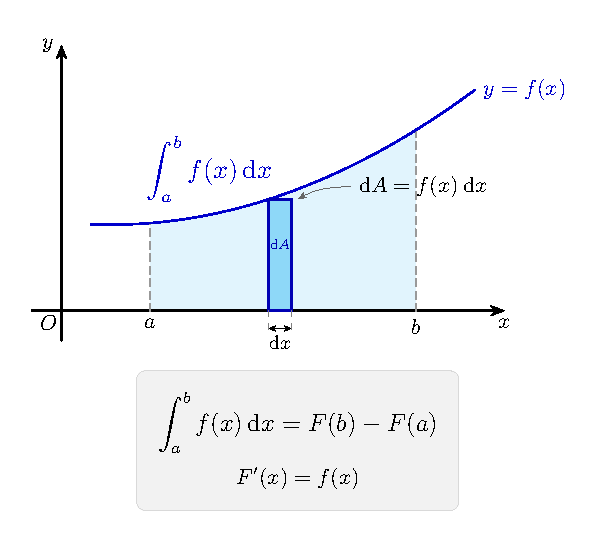
\includegraphics[width=0.6\linewidth]{figure/fig3.2}
	\caption[牛顿-莱布尼兹公式]{牛顿-莱布尼兹公式}
	\label{fig:3.2}
\end{figure}

\subsection{平面 Green 公式}

在二维区域 $D$ 中, 设一次形式为
\begin{equation}
	\omega=P\,\dif x+Q\,\dif y.
\end{equation}
则
\[
\dif\omega
=
\dif P\wedge \dif x+\dif Q\wedge \dif y.
\]
由于
\[
\dif P=P_x\,\dif x+P_y\,\dif y,
\]
\[
\dif Q=Q_x\,\dif x+Q_y\,\dif y,
\]
所以
\[
\dif\omega
=
(P_x\,\dif x+P_y\,\dif y)\wedge \dif x
+
(Q_x\,\dif x+Q_y\,\dif y)\wedge \dif y.
\]
利用
\[
\dif x\wedge \dif x=0,
\qquad
\dif y\wedge \dif y=0,
\qquad
\dif y\wedge \dif x=-\dif x\wedge \dif y,
\]
得到
\[
\dif\omega
=
(Q_x-P_y)\dif x\wedge \dif y.
\]
广义 Stokes 公式给出
\begin{equation}
	\int_D(Q_x-P_y)\dif x\dif y
=
\oint_{\partial D}P\,\dif x+Q\,\dif y.
\end{equation}
这就是平面 Green 公式. 
\begin{figure}
	\centering
	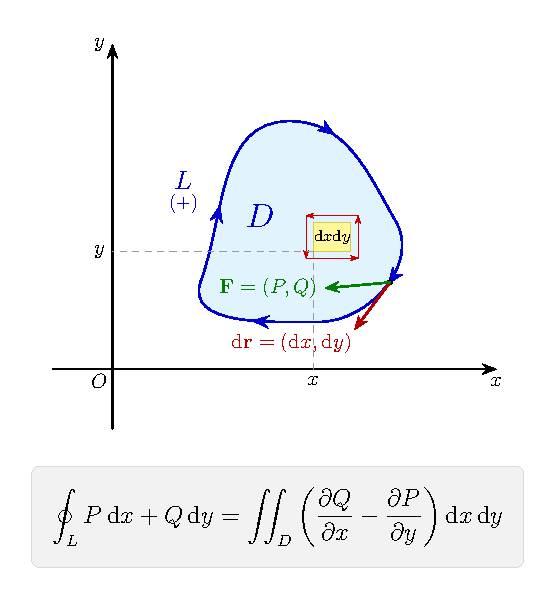
\includegraphics[width=0.5\linewidth]{figure/fig3.3}
	\caption[Green公式]{Green公式}
	\label{fig:3.3}
\end{figure}

\begin{example}{用微分形式推出 Green 公式的被积表达式}{3,3}
设平面区域上的一次形式为
\[
\omega=P\,\dif x+Q\,\dif y.
\]
求 $\dif\omega$, 并说明它与 Green 公式中的面积分被积函数的关系.
\begin{solution}
	由外微分的 Leibniz 规则和 $\dif^{2}x=\dif^{2}y=0$, 有
	\[
	\dif\omega
	=
	\dif P\wedge\dif x+
	\dif Q\wedge\dif y.
	\]
	又因为
	\[
	\dif P=P_x\,\dif x+P_y\,\dif y,
	\qquad
	\dif Q=Q_x\,\dif x+Q_y\,\dif y,
	\]
	所以
	\[
	\dif\omega
	=
	P_y\,\dif y\wedge\dif x+Q_x\,\dif x\wedge\dif y.
	\]
	利用 $\dif y\wedge\dif x=-\dif x\wedge\dif y$, 得到
	\[
	\dif\omega
	=
	(Q_x-P_y)\,\dif x\wedge\dif y.
	\]
	因此 Green 公式中的面积分被积函数 $Q_x-P_y$ 正是一次形式 $\omega$ 的外微分系数. 
\end{solution} 
\end{example}

\subsection{三维 Stokes 公式}

设三维空间中的向量场为 $\bm{A}$, 其对应一次形式为
\[
A^\flat=A_i \dif x^i.
\]
则
\[
\dif A^\flat
\]
是一个二次形式. 由
\[
(\nabla\times\bm{A})^\flat=*\dif A^\flat
\]
可知, $\dif A^\flat$ 对应旋度的通量形式. 

广义 Stokes 公式给出
\begin{equation}
	\int_S \dif A^\flat
=
\oint_{\partial S}A^\flat.
\end{equation}
写成传统向量形式, 就是
\begin{equation}
	\int_S(\nabla\times\bm{A})\cdot \dif\bm{S}
=
\oint_{\partial S}\bm{A}\cdot \dif\bm{l}.
\end{equation}
\subsection{三维Gauss公式}

设向量场 $\bm{A}$ 对应一次形式 $A^\flat$. 通量二形式为
\[
*A^\flat.
\]
由散度公式
\[
(\nabla\cdot\bm{A})\mathrm{vol}
=
\dif(*A^\flat),
\]
可知 $\dif(*A^\flat)$ 是散度对应的体积形式. 

广义 Stokes 公式给出
\begin{equation}
	\int_V \dif(*A^\flat)
=
\oint_{\partial V}*A^\flat.
\end{equation}
写成传统向量形式, 就是
\begin{equation}
	\int_V\nabla\cdot\bm{A}\,\dif V
=
\oint_{\partial V}\bm{A}\cdot \dif\bm{S}.
\end{equation}
因此, Gauss公式和 Stokes 公式不是两个孤立的定理, 而是同一个广义 Stokes 公式在不同维数和不同阶数微分形式上的表现. 
\begin{figure}[h]
	\centering
	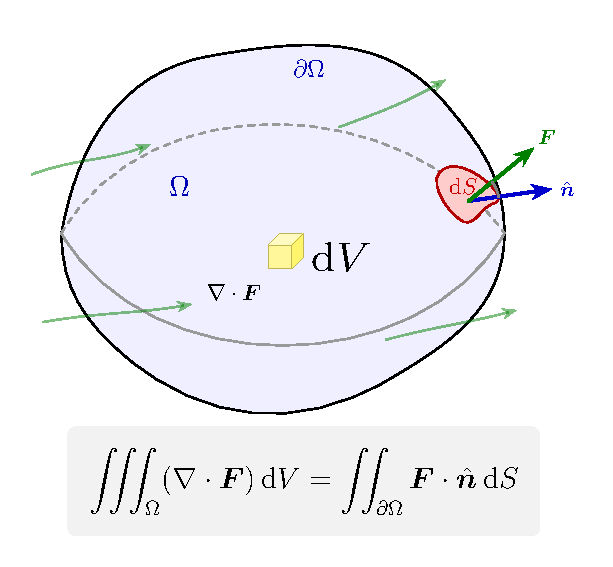
\includegraphics[width=0.5\linewidth]{figure/fig3.4}
	\caption[Gauss散度定理]{Gauss散度定理}
	\label{fig:3.4}
\end{figure}

\section{本章小结}

本章的核心思想是: 微分形式天然适合描述积分对象, 外微分天然适合描述边界与内部之间的关系. 

标量场是 $0$-形式. 对标量场 $f$, 外微分为
\[
\dif f=\partial_i f\,\dif x^i.
\]
一次形式写作
\[
\omega=\omega_i \dif x^i.
\]
它适合沿曲线积分. 

二次形式写作
\[
\eta=\frac{1}{2}\eta_{ij}\dif x^i\wedge \dif x^j.
\]
它适合在曲面上积分. 

三次形式写作
\[
\Omega=F\,\dif x^1\wedge \dif x^2\wedge \dif x^3.
\]
它适合在三维区域上积分. 

外微分满足
\[
\dif^{2}=0.
\]
这统一了向量分析中的两个恒等式: 
\[
\nabla\times(\nabla f)=0,
\]
\[
\nabla\cdot(\nabla\times\bm{A})=0.
\]
在带度规和取向的三维空间中, Hodge 星号把 $p$-形式对应到 $(3-p)$-形式. 借助度规, 向量和一次形式可以通过升降指标互相对应: 
\[
A^\flat=A_i \dif x^i,
\qquad
A_i=g_{ij}A^j.
\]
传统向量分析中的三个基本微分算符可以写成: 
\[
(\nabla f)^\flat=\dif f,
\]
\[
(\nabla\times\bm{A})^\flat=*\dif A^\flat,
\]
\[
(\nabla\cdot\bm{A})\mathrm{vol}=\dif(*A^\flat).
\]
广义 Stokes 公式为
\[
\int_M \dif\omega
=
\int_{\partial M}\omega.
\]
统一了微积分基本定理、Green 公式、Stokes 公式和 Gauss 公式. 